% Options for packages loaded elsewhere
\PassOptionsToPackage{unicode}{hyperref}
\PassOptionsToPackage{hyphens}{url}
%
\documentclass[
  parskip,
  oneside]{scrreprt}
\author{}
\date{\vspace{-2.5em}}

\usepackage{amsmath,amssymb}
\usepackage{lmodern}
\usepackage{iftex}
\ifPDFTeX
  \usepackage[T1]{fontenc}
  \usepackage[utf8]{inputenc}
  \usepackage{textcomp} % provide euro and other symbols
\else % if luatex or xetex
  \usepackage{unicode-math}
  \defaultfontfeatures{Scale=MatchLowercase}
  \defaultfontfeatures[\rmfamily]{Ligatures=TeX,Scale=1}
\fi
% Use upquote if available, for straight quotes in verbatim environments
\IfFileExists{upquote.sty}{\usepackage{upquote}}{}
\IfFileExists{microtype.sty}{% use microtype if available
  \usepackage[]{microtype}
  \UseMicrotypeSet[protrusion]{basicmath} % disable protrusion for tt fonts
}{}
\makeatletter
\@ifundefined{KOMAClassName}{% if non-KOMA class
  \IfFileExists{parskip.sty}{%
    \usepackage{parskip}
  }{% else
    \setlength{\parindent}{0pt}
    \setlength{\parskip}{6pt plus 2pt minus 1pt}}
}{% if KOMA class
  \KOMAoptions{parskip=half}}
\makeatother
\usepackage{xcolor}
\IfFileExists{xurl.sty}{\usepackage{xurl}}{} % add URL line breaks if available
\IfFileExists{bookmark.sty}{\usepackage{bookmark}}{\usepackage{hyperref}}
\hypersetup{
  hidelinks,
  pdfcreator={LaTeX via pandoc}}
\urlstyle{same} % disable monospaced font for URLs
\usepackage{color}
\usepackage{fancyvrb}
\newcommand{\VerbBar}{|}
\newcommand{\VERB}{\Verb[commandchars=\\\{\}]}
\DefineVerbatimEnvironment{Highlighting}{Verbatim}{commandchars=\\\{\}}
% Add ',fontsize=\small' for more characters per line
\usepackage{framed}
\definecolor{shadecolor}{RGB}{248,248,248}
\newenvironment{Shaded}{\begin{snugshade}}{\end{snugshade}}
\newcommand{\AlertTok}[1]{\textcolor[rgb]{0.94,0.16,0.16}{#1}}
\newcommand{\AnnotationTok}[1]{\textcolor[rgb]{0.56,0.35,0.01}{\textbf{\textit{#1}}}}
\newcommand{\AttributeTok}[1]{\textcolor[rgb]{0.77,0.63,0.00}{#1}}
\newcommand{\BaseNTok}[1]{\textcolor[rgb]{0.00,0.00,0.81}{#1}}
\newcommand{\BuiltInTok}[1]{#1}
\newcommand{\CharTok}[1]{\textcolor[rgb]{0.31,0.60,0.02}{#1}}
\newcommand{\CommentTok}[1]{\textcolor[rgb]{0.56,0.35,0.01}{\textit{#1}}}
\newcommand{\CommentVarTok}[1]{\textcolor[rgb]{0.56,0.35,0.01}{\textbf{\textit{#1}}}}
\newcommand{\ConstantTok}[1]{\textcolor[rgb]{0.00,0.00,0.00}{#1}}
\newcommand{\ControlFlowTok}[1]{\textcolor[rgb]{0.13,0.29,0.53}{\textbf{#1}}}
\newcommand{\DataTypeTok}[1]{\textcolor[rgb]{0.13,0.29,0.53}{#1}}
\newcommand{\DecValTok}[1]{\textcolor[rgb]{0.00,0.00,0.81}{#1}}
\newcommand{\DocumentationTok}[1]{\textcolor[rgb]{0.56,0.35,0.01}{\textbf{\textit{#1}}}}
\newcommand{\ErrorTok}[1]{\textcolor[rgb]{0.64,0.00,0.00}{\textbf{#1}}}
\newcommand{\ExtensionTok}[1]{#1}
\newcommand{\FloatTok}[1]{\textcolor[rgb]{0.00,0.00,0.81}{#1}}
\newcommand{\FunctionTok}[1]{\textcolor[rgb]{0.00,0.00,0.00}{#1}}
\newcommand{\ImportTok}[1]{#1}
\newcommand{\InformationTok}[1]{\textcolor[rgb]{0.56,0.35,0.01}{\textbf{\textit{#1}}}}
\newcommand{\KeywordTok}[1]{\textcolor[rgb]{0.13,0.29,0.53}{\textbf{#1}}}
\newcommand{\NormalTok}[1]{#1}
\newcommand{\OperatorTok}[1]{\textcolor[rgb]{0.81,0.36,0.00}{\textbf{#1}}}
\newcommand{\OtherTok}[1]{\textcolor[rgb]{0.56,0.35,0.01}{#1}}
\newcommand{\PreprocessorTok}[1]{\textcolor[rgb]{0.56,0.35,0.01}{\textit{#1}}}
\newcommand{\RegionMarkerTok}[1]{#1}
\newcommand{\SpecialCharTok}[1]{\textcolor[rgb]{0.00,0.00,0.00}{#1}}
\newcommand{\SpecialStringTok}[1]{\textcolor[rgb]{0.31,0.60,0.02}{#1}}
\newcommand{\StringTok}[1]{\textcolor[rgb]{0.31,0.60,0.02}{#1}}
\newcommand{\VariableTok}[1]{\textcolor[rgb]{0.00,0.00,0.00}{#1}}
\newcommand{\VerbatimStringTok}[1]{\textcolor[rgb]{0.31,0.60,0.02}{#1}}
\newcommand{\WarningTok}[1]{\textcolor[rgb]{0.56,0.35,0.01}{\textbf{\textit{#1}}}}
\usepackage{longtable,booktabs,array}
\usepackage{calc} % for calculating minipage widths
% Correct order of tables after \paragraph or \subparagraph
\usepackage{etoolbox}
\makeatletter
\patchcmd\longtable{\par}{\if@noskipsec\mbox{}\fi\par}{}{}
\makeatother
% Allow footnotes in longtable head/foot
\IfFileExists{footnotehyper.sty}{\usepackage{footnotehyper}}{\usepackage{footnote}}
\makesavenoteenv{longtable}
\usepackage{graphicx}
\makeatletter
\def\maxwidth{\ifdim\Gin@nat@width>\linewidth\linewidth\else\Gin@nat@width\fi}
\def\maxheight{\ifdim\Gin@nat@height>\textheight\textheight\else\Gin@nat@height\fi}
\makeatother
% Scale images if necessary, so that they will not overflow the page
% margins by default, and it is still possible to overwrite the defaults
% using explicit options in \includegraphics[width, height, ...]{}
\setkeys{Gin}{width=\maxwidth,height=\maxheight,keepaspectratio}
% Set default figure placement to htbp
\makeatletter
\def\fps@figure{htbp}
\makeatother
\setlength{\emergencystretch}{3em} % prevent overfull lines
\providecommand{\tightlist}{%
  \setlength{\itemsep}{0pt}\setlength{\parskip}{0pt}}
\setcounter{secnumdepth}{5}
\newlength{\cslhangindent}
\setlength{\cslhangindent}{1.5em}
\newlength{\csllabelwidth}
\setlength{\csllabelwidth}{3em}
\newlength{\cslentryspacingunit} % times entry-spacing
\setlength{\cslentryspacingunit}{\parskip}
\newenvironment{CSLReferences}[2] % #1 hanging-ident, #2 entry spacing
 {% don't indent paragraphs
  \setlength{\parindent}{0pt}
  % turn on hanging indent if param 1 is 1
  \ifodd #1
  \let\oldpar\par
  \def\par{\hangindent=\cslhangindent\oldpar}
  \fi
  % set entry spacing
  \setlength{\parskip}{#2\cslentryspacingunit}
 }%
 {}
\usepackage{calc}
\newcommand{\CSLBlock}[1]{#1\hfill\break}
\newcommand{\CSLLeftMargin}[1]{\parbox[t]{\csllabelwidth}{#1}}
\newcommand{\CSLRightInline}[1]{\parbox[t]{\linewidth - \csllabelwidth}{#1}\break}
\newcommand{\CSLIndent}[1]{\hspace{\cslhangindent}#1}
\usepackage[utf8]{inputenc}
\usepackage[T1]{fontenc}
\usepackage{lmodern}
\usepackage[onehalfspacing]{setspace}
\usepackage[left=2.50cm, right=2.50cm, top=2.50cm, bottom=2.50cm, bindingoffset=10mm, includehead, includefoot]{geometry}
\usepackage[headsepline]{scrlayer-scrpage}
\usepackage{url}
\usepackage[backend=biber, style=authoryear, giveninits=true, maxbibnames=99, uniquename=init, maxcitenames=2, hyperref=true, date=year]{biblatex}
\usepackage{xpatch}
\usepackage{csquotes}
\usepackage{amsmath}
\usepackage{listings}
\usepackage{booktabs}
\usepackage{longtable}
\usepackage{multirow}
\usepackage{rotating}
\usepackage{subfigure}
\usepackage{graphicx}
\usepackage{float}
\usepackage{acronym}
\usepackage{lipsum}
\usepackage{scrhack}
\emergencystretch=50pt
\clubpenalty = 10000
\widowpenalty = 10000
\displaywidowpenalty = 10000
\automark[section]{chapter}
\renewcommand*{\chaptermarkformat}{}
\renewcommand*{\sectionmarkformat}{}
\setkomafont{title}{\sffamily}
\setkomafont{disposition}{\usekomafont{title}}
\setkomafont{author}{\usekomafont{title}}
\setkomafont{date}{\usekomafont{title}}
\setkomafont{caption}{\sffamily\small}
\setkomafont{captionlabel}{\usekomafont{caption}\bfseries\small}
\setkomafont{pagehead}{\normalfont\scshape}
\ifLuaTeX
  \usepackage{selnolig}  % disable illegal ligatures
\fi

\begin{document}

\begin{titlepage}
\centering
    {\Large Ruprecht-Karls-University Heidelberg\\
        Faculty for Life Sciences\\
        Molecular Biotechnology\\}

    {\vspace{\stretch{2}}}
    {\usekomafont{title}

        {\Huge Thyorid cancer: Comparison of linar model and neuronal network (xxx)}

        {\Huge 3-Sätze-Zusammenfassung}

        {\Huge sfsf}

    }

    \vspace{\stretch{2}}
    {\Large Data Science Project SoSe 2022}

    \vspace{\stretch{2}}

    {\Large
        \begin{tabular}{rl}
            Autoren & Anna Lange, David Matuschek, Jakob Then, Maren Schneider\\
            Geburtsort & Heidelberg\\
            Abgabetermin &20.07.2022\\
        \end{tabular}
    }

    \vspace{\stretch{1}}

\end{titlepage}

\tableofcontents

\renewcommand\abstractname{\Large Acknowledgments}
\begin{abstract}
In the recent years bioinformatic methods became a tool of utmost importance in medical research. To define specific genes and pathways in different cancer types or histological types pan-cancer analysis are done. A focused analysis is done to specify different subcategories within a certain cancer type and to identify targets for targeted therapy. The main methods in identifying up- or down-regulated pathways are GSEA and GSVA. GSVA of TCGA expression data reveals four clusters of cancer types, which are defined by different histological types like glioblastoma and adenocarcinoma. The histological types therefore seems to correlate with a specific set of pathways being especially enriched in certain cancer types. Furthermore, a GSVA of Thyroid cancer expression data shows that thyroid carcinogenisis is associated with the up-regulation of proliferative signalling pathways like the hedgehog pathway and alpha6beta4 integrin signaling pathway and associated pathways such as IL-36 signaling. It also showed the down-regulation of a pathway that is associated with an increased MAP-kinase acitivity. It is based on those proliferative signalling pathways that three subclusters form inside of the THCA patients from the pan-cancer data. One THCA subtype that could be linked to the follicular histological subtype is defined by increased mTOR and MAPK acitivity, while having low alpha6beta4 activity. In contrast another THCA subtype is defined by a low mTOR and MAPK activity, but a high alpha6beta4 activity. The third THCA subtype is linked to enhanced activity of both of these proliferative signalling pathways. These results promise better results is treatment, as a more percise diagnosis of the distinct THCA subtypse is possible
To improve the understanding of THCA and thereby hopefully improve patients prognosis, this project focuses on finding genes that have a significantly different expression in THCA compared to other cancers and especially to normal tissue.
\end{abstract}

\renewcommand\abstractname{\Large Abstract}
\begin{abstract}
Thank You
\end{abstract}

\hypertarget{introduction}{%
\chapter{Introduction}\label{introduction}}

In 2019 230,000 cancer deaths were documented in
Germany\footnote{ https://www.krebsinformationsdienst.de/tumorarten/grundlagen/krebsstatistiken.php}.
To detect and fight tumors, the development of new treatment and
detection methods is essential. For that it is beneficial to find a
similarities in mutational causes across different tumors by using
transcriptomic profiling methods like RNA-seq. In transcriptomic
profiling all the RNA that has been generated by transcription of a
cells DNA is sequenced (Alberts and Walter, 2015).

\hypertarget{hallmarks-of-cancer}{%
\section{Hallmarks of cancer}\label{hallmarks-of-cancer}}

The Hallmarks of Cancer are properties of tumors, that can be detected
in each tumor. Among others those are: resisting cell death, inducing
angiogenesis, enabling replicative immortality, activating invasion and
metastasis evading growth suppressors were the first detected hallmarks
(Hanahan and Weinberg, 2011).

\hypertarget{histological-tumor-types}{%
\section{Histological tumor types}\label{histological-tumor-types}}

The observed tumors can be classified into different histological types.
Carcinoma, which can be further subcategorized into adenocarcinomas,
squamous cell carcinoma, transitional cell carcinoma. Carcioma derive
from epithelial cells. Melanoma are skin tumors, sarcoma derive from
connective or supportive tissue cells, glioblastoma are brain tumors and
leukemia affect bloodcells (Alberts and Walter, 2015).

\hypertarget{rna-sequencing}{%
\section{RNA-sequencing}\label{rna-sequencing}}

RNA-sequencing (RNA-seq) is performed by cleaning of RNA, fragmentation,
translation of RNA to cDNA, sequencing of cDNA and comparison with a
reference genome. The advantage of RNA-seq is that it includes
information about gene expression that is especially important in the
analysis of tumors such as epigenetic changes (e.g.~epigenetic gene
silencing) or fusion proteins (Alberts and Walter, 2015).

The results from RNA-seq used for the analysis stem from data from the
cancer genome atlas (TCGA).

\hypertarget{thyroid-carcinoma}{%
\section{Thyroid carcinoma}\label{thyroid-carcinoma}}

Thyroid carcinoma (THCA) incidence increased dramatically over the past
few years (Cabanillas \emph{et al.}, 2016). The main tasks of the
thyroid gland are synthesizing hormones and regulating body temperate
and metabolism (Tsibulnikov \emph{et al.}, 2020). Most THCA derive from
thyroid cells and result in the thyroid gland losing its function.
Thyroid cancer can occur in two different types, differentiated and
undifferentiated thyroid cancer. Those two types again have histological
subtypes. Papillary thyroid cancer (PTC), the most common THCA,
follicular thyroid cancer (FTC) and a tall cell variant (TCV) are
subtypes of differentiated thyroid cancer (DTC). Medullary and
anaplastic thyroid cancer are subtypes of undifferentiated thyroid
cancer (UTC). Prevalence of DTCs is clearly higher than of UTCs (Prete
\emph{et al.}, 2020). Regarding the presented DTCs, PTCs have the best
clinical prognosis (Lin, 2007), while TCV cancers have the worst
clinical outcome (Coca-Pelaz \emph{et al.}, 2020). Therefore, the
detection of the tumor type would be important and for more specific
therapy options. Even though, all thyroid cancers are treated with
thyroidectomy and radioactive iodine, the additional therapy differs for
each histological type (Kant \emph{et al.}, 2020).

\hypertarget{integrin}{%
\subsubsection{Integrin}\label{integrin}}

Integrin is a cellular adhesion molecule, that binds to laminin in the
extracellular matrix (Liberzon \emph{et al.}, 2015). Together with other
proteins they form hemidesmosomes. Thereby, integrin is essential for
the integrity between cells. An important step in the development of
malignant cancer is the invasion into healthy tissue. Thus, the
detachment of the extracellular matrix from of the surrounding cells is
essential and alterations of integrin are very common in cancer cells
(\textbf{Integrin2?}).

\hypertarget{computational-tools}{%
\section{Computational tools}\label{computational-tools}}

\hypertarget{gene-set-enrichment-analysis}{%
\subsection{Gene Set Enrichment
Analysis}\label{gene-set-enrichment-analysis}}

To analyse how the activity of a gene set differs between two sets of
gene expression data, a Gene Set Enrichment Analysis (GSEA) is
performed. For this, the genes in the expression data have to be ranked
decreasingly by a certain metric. Such metrics can include the log2 fold
change between the sample expression data and a reference set or the
associated p-values for each gene. After ranking, a cumulative sum of
all expression values in the ranked sample is computed. If a gene is
present in the gene set to be analysed the expression value of that gene
is added to the running sum. However, if the current gene does not lie
in the gene set the value is subtracted. The extremum of this running
sum is termed the enrichment score of the gene set. It is positive if
the gene set is overexpressed in the sample compared to the reference
data and negative vice versa. (Reimand \emph{et al.}, 2019)

\hypertarget{gene-set-variation-analysis}{%
\subsection{Gene Set Variation
Analysis}\label{gene-set-variation-analysis}}

The Gene Set Variation Analysis (GSVA) is performed with the same
intention as the GSEA - to analyse the gene set activities in gene
expression data. However, no reference data is required to successfully
perform GSVA. There are various approaches to GSVA, one of them is
performed by \[@GSVA\] by following five steps. First, the cumulative
density distribution of a gene over all samples is estimated. Then the
expression statistic of a gene in a sample based on the cumulative
density distribution is calculated to bring all of the expression values
to the same level. The third step is to rank the genes based on the
expression statistic and to normalize the ranks with z-transformation.
Lastly, the enrichment score is computed based on the obtained ranked
list by calculating the Kolmogorov-Smirnov-like rank statistic for each
gene set. \[@GSVA\]

\hypertarget{principal-component-analysis-xxx-quelle}{%
\subsection{Principal component analysis xxx
QUELLE}\label{principal-component-analysis-xxx-quelle}}

A Principal component analysis (PCA) is used to alter the coordinates of
a given dataset to its eigenvectors. This matrix rotation results in a
new set of basis vectors called principal components (PCs) - the
eigenvectors - that are orthogonal and show little correlation. Sorting
the PCs by their associated eigenvalue, sthe PCs explaining the most
variance can easily be identified, as they have the highest eigenvalue.
By displaying the data set in a coordinate system span by the n most
variant PCs, the dimensionalty of the dataset is reduced to
\(\mathbb{R}^n\) with the lowest loss in variance.

\hypertarget{uniform-manifold-approximation-and-projection-for-dimension-reduction}{%
\subsection{Uniform Manifold Approximation and Projection for Dimension
Reduction}\label{uniform-manifold-approximation-and-projection-for-dimension-reduction}}

The Uniform manifold approximation and projection for dimension
reduction (UMAP) is a method to reduce the dimension of a
multidimensional data set. Compared to PCA, UMAP preserves the global
structure of the data better and is much faster than other comparable
techniques like t-SNE (Maaten and Hinton, 2008). The algorithm starts by
setting up a high-dimensional graph representation of the data. From
each data point, a radius is extended and when two radii come into
contact the points are connected in the graph. The radius is chosen
individually for each point based on the distance to the nearest
neighbor. The algorithm goes on until k points are connected or n
iterations are reached. The resulting clustered high-dimensional graph
is then optimized for a visualization in low-dimensions. A disadvantage
of UMAP is that although the overall structure is conserved, the
distances between the individual points are not proportional to the real
distance in the data set. This arises from the non-linear dimensional
reduction. (Sharma \emph{et al.}, 2021)

\hypertarget{jaccard-index}{%
\subsection{Jaccard index}\label{jaccard-index}}

The Jaccard index is the intersection, divided by the union of two sets.
Therefore, it can be used to identify the similarity of the sets.

\hypertarget{pan-cancer-analysis}{%
\section{Pan Cancer Analysis}\label{pan-cancer-analysis}}

For the pan cancer analysis 3 data sets are provided. One containing
expression data of 60,000 genes in 10,000 tumor patients. Another one
contains clinical annotations concerning those patients and the last one
contains hallmark pathways and their included genes. In the following
analysis the data is cleaned by removing NAs, biotype filtering and
low-variance filtering. After that a descriptive analysis is performed.
After that a gene set variation analysis to detect significantly altered
pathways compared to the other pathways in tumor tissue and a linear
regression analysis is performed to predict pathway activity based on
other pathways??? xxx Furthermore a neuronal network is built to improve
prediction.

\hypertarget{focused-analysis-on-thca-patients}{%
\section{Focused analysis on THCA
patients}\label{focused-analysis-on-thca-patients}}

An analysis of THCA patients is performed. This analysis is done on a
data set containing the gene expression data of 60 patients in tumor an
normal tissue and their clinical annotations. First the data is cleaned
and described like the pan cancer data to prepare the data for the gene
set variation analysis. GSVA is performed on the THCA data in the bigger
pan cancer data set, to confirm results from the smaller data set. In
this analysis a linear regression analysis is performed to predict the
activity of other pathways based on thyroxine biosynthesis (nicht
mehr!!!!) xxx. A better prediction can be achieved with a neuronal
network.

\hypertarget{linear-regression-analysis}{%
\section{Linear regression analysis}\label{linear-regression-analysis}}

Linear regression is a statistical model that uses measurable values to
predict an outcome. For this purpose, a linear function serves as basis
to built the linear regression equation (Lunt, 2013). In gene expression
data analysis a linear regression equation can be used to predict the
activity of one gene (or pathway) by the activity of another.

\hypertarget{neural-network}{%
\section{Neural network}\label{neural-network}}

A neural network was performed using the package ``neuralnet'' (Fritsch
\emph{et al.}, 2019). In general, a deep learning network consists of an
input layer, multiple hidden layers and an output layer (Riedmiller).
Each one consisting of various neurons. The input layer contains as much
neurons as input numbers are given for each sample. The output layer
contains as much neurons as possible outputs. The number of neurons in
each hidden layer and the number of hidden layers vary and will be
determined for the best results. Based on the input numbers in the input
layer, the number of each neuron of the next layer is determined, based
on a linear regression model composed of the input data, weights, and
bias.

\[
\sum_{i=1} ^{n} w_i x_i + bias
\]

\emph{n} is the number of input neurons and \emph{w} the weight.

To obtain numbers in the range of 0 and 1, a min/max-scaling is
performed on the input data. Furthermore, the optimal number of neurons
per layer and the best random weights and biases for the first sample
must be determined. This is done because some weights and biases may
result in finding a local, but not global minimum of the cost function.
After determining the random weights and bias, which resulted in a
random output for the first sample, the cost function is calculated. To
minimize the cost, resilient backpropagation with weight backtracking is
used. Therefore, the gradient function of the cost function is
determined. In resilient backpropagation, only the sign of the derivate
is used, to avoid harmful effects of its magnitude. For minimizing the
cost function, the ideal weights and biases are determined, based on the
input and the expected output. (Theoretisch kann man hier ja noch
schreiben, dass nicht nur das Erreichen des Minimums, sondern auch die
Geschwindigkeit für das Erreichen des Minimums relevant sind) xxx. For
the next samples those steps are repeated to reach the minimum of the
cost function.

\[
Cost function = \frac {1}{2m} \sum_{i=1} ^{m} (x - y)^2
\]

\emph{m} is the number of samples, \emph{y} the output and \emph{x} the
expected output.

\hypertarget{materials-and-methods}{%
\chapter{Materials and Methods}\label{materials-and-methods}}

For the means of this project two separate analysis are performed: a
pan-cancer analysis focusing on differences between cancer types and a
focused analysis investigating THCA.

\hypertarget{description-of-the-underlying-data}{%
\section{Description of the underlying
data}\label{description-of-the-underlying-data}}

For the analysis four data sets were provided. For pan-cancer analysis a
gene expression data frame with normalized and log2 transformed bulk
RNA-seq expression data for 60,489 genes in 9741 patients with 33
different forms of cancer was used. The data was derived from The Cancer
Genome Atlas (TCGA). Complementing the TCGA expression data is an
annotation dataframe with 37 clinical annotations regarding tumor type,
tumor stage, gender, age, etc. for all patients.

The third object is a list containing five lists for the focused
analysis, one list for each tumor type (BRCA, KIRC, LUAD, PRAD, THCA).
For our focused analysis, the only the THCA data were used. The THCA
list consists of three data frames: The first two contain normalized and
log2 transformed bulk RNA-seq expression data for 19,624 genes in 59
THCA patients for carcinogenic and homeostatic tissue. The third
dataframe complementes the data with the respective clinical
annotations.

The last object contains 46 pathways associated with the hallmarks of
cancer in form of a list of string vectors.

\hypertarget{metabolic-pathway-selection}{%
\section{Metabolic pathway
selection}\label{metabolic-pathway-selection}}

To perform enrichment analysis later on, 6366 canonical pathways were
selected from the Molecular Signatures Database (MSigDB)\[@msigdb\] with
the \texttt{msigdbr::msigdbr()} function. As not to introduce a bias
during enrichment analysis, the similarity of MSigDB pathways among
themselves as well as with the hallmark pathways was computed with the
Jaccard index. Pathways with a Jaccard index greater than the
1\(\sigma\) range were discarded.

\hypertarget{preprocessing-of-expression-data}{%
\section{Preprocessing of expression
data}\label{preprocessing-of-expression-data}}

\hypertarget{data-cleaning}{%
\subsection{Data cleaning}\label{data-cleaning}}

All expression data were checked for missing values with the
\texttt{na.omit()} function. Subsequently, low variance filtering was
performed for TCGA and THCA tumor expression data. The variances of
expression were computed for every gene across all samples and then,
genes with variances blow a threshold were discarded to reduce
dimensionality.

\hypertarget{biotype-filtering}{%
\subsection{Biotype filtering}\label{biotype-filtering}}

Next, biotype filtering was performed for pan-cancer and THCA expression
data to reduce dimensionality further. Only genes sharing biotypes with
the hallmark pathways were kept for the the following analysis. The
biotypes of the genes were retrieved using the \texttt{biomart::getBM()}
function from the biomaRt package (Durinck \emph{et al.}, 2009). To
allow for an appropriate comparison within all pathways, only MSigDB
pathways where over 99\% of their respective genes were present in the
filtered expression data were selected as final pathways.

\hypertarget{methods-for-descriptive-analysis}{%
\section{Methods for descriptive
analysis}\label{methods-for-descriptive-analysis}}

\hypertarget{mean-variance-plot}{%
\subsection{Mean-variance plot}\label{mean-variance-plot}}

In a mean-variance plot the variance is plotted over the mean of
expression values of single genes across all patients. Thus, the
variance and mean were calculated for each gene in the THCA expression
data. The final plot was created with the package ggplot2 \ref{ggplot2}.

\hypertarget{kann-raus-m.m.n-violin-plot}{%
\subsection{KANN RAUS m.M.n Violin
plot}\label{kann-raus-m.m.n-violin-plot}}

To check the distribution of a data set and compare it with other data
sets violin plots are used. Based on how similar the violin plots are,
it can be implied that the data is normalized. Violin plots are tilted
and mirrored density plots of gene expression values. The y-axis shows
the gene expression value and the x-axis shows the amount of genes with
a certain gene expression value.

\hypertarget{jaccard-index-1}{%
\subsection{Jaccard-Index}\label{jaccard-index-1}}

The Jaccard-Index is a method to describe the similarity between two
quantities. To compute it, the intersection of all gene ENSEMBL-IDs from
two compared pathways was divided by their union. We used this method to
determine the degree in which pathways are similar to each other.

\hypertarget{volcano-plot}{%
\subsection{Volcano plot}\label{volcano-plot}}

A volcano plot is used to identify genes displaying significantly
different expression in carcinogenic versus homeostatic tissues. First,
the log2 fold change (Log2FC) is calculated for each gene across all
samples in the THCA expression data in the following way:

\[
log2FC = mean(normal tissue) - mean(tumor tissue)
\]Next, a two-sided t-test was performed with the \texttt{t.test()}
function to determine the significance of a difference in expression. To
avoid the accumulation of type one errors, a Bonferroni correction was
performed. n is the number of genes in the cleaned data set for focused
analysis:

\[
\alpha = \frac{0.025}{n}
\]

In the volcano plot the -log10 of the calculated p-values is plotted
against die Log2FC. Genes with a lower p-value than the corrected
significance level \(\alpha\) are significantly differently expressed.
If the Log2FC is additionally positive, the genes are significantly
overexpressed in tumor tissue, if the Log2FC is negative, the genes are
significantly underexpressed in tumor tissue.

\hypertarget{dimension-reduction-and-pathway-enrichment-analysis}{%
\section{Dimension reduction and pathway enrichment
analysis}\label{dimension-reduction-and-pathway-enrichment-analysis}}

The GSEA was used to identify enriched pathways in THCA tumor tissue.
Here, GSEA was performed with the package ``fgsea'' (Korotkevich
\emph{et al.}, 2019). First, the expression values were ranked
decreasingly by log2FC for every patient. Log2FC was chosen as the
ranking metric as it easy to compute and shows a high sensitivity.
\textbf{xxx Quelle: Ranking metrics in gene set enrichment analysis: do
they matter?} Secondly, using the ranked log2FC vectors, the enrichment
score of each pathway was calculated for each patient with the
\texttt{fgseamultilevel()} function.

As no normal tissue reference data was provided for the TCGA expression
data, pathway activities were computed via GSVA. The analysis was
performed with the \texttt{gsva()} function from the ``GSVA'' package
(Hänzelmann \emph{et al.}, 2013). To give a general overview over the
differences in expression of THCA and homeostatic thyroid tissue GSVA,
the THCA expression data were also analysed by GSVA. To do so, tumor and
normal expression data were combined into a singular dataframe of which
enrichment scores were computed with \texttt{gsva()}. Than, the GSVA
data was split again and the log2FC between the two matrices was
computed and taken as pathway activity.

PCA was performed to provide an uncorrelated dataset for the subsequent
UMAP. For the TCGA GSVA pathway activity data the \texttt{prcomp()}
function was used. To verify the results, PCA was performed on TCGA
expression data, as well. In this case \texttt{Seurat::RunPCA()} from
the Seurat package was used to minimized computation times. \textbf{xxx
Quelle: seurat package}

UMAP analysis was used to identify and visualize clusters in TCGA GSVA
and expression data. This was achieved with the \texttt{umap()} function
from the package ``umap'' \[@umap\] running on all PCs from TCGA GSVA
ans expression data.

\hypertarget{regression-analysis}{%
\section{Regression analysis}\label{regression-analysis}}

\hypertarget{linear-regression}{%
\subsection{Linear Regression}\label{linear-regression}}

A linear regression analysis is performed to predict the activity of xxx
based on the activity of the other pathways.

Firstly, the correlation of the pathways for predicting is checked, only
pathways with a low correlation were kept. In the next step, the
variance is checked, 80\% of the genes with low variance were omitted.

For the regression analysis only 20\% of the pathways were used, to only
use significant pathways.

The regression analysis was tested by

\hypertarget{neuronal-network}{%
\subsection{Neuronal Network}\label{neuronal-network}}

A neural network was used to predict the activity of
REACTOME\_INTERLEUKIN\_36\_PATHWAY based on the activity of other
pathways. Therefore, the network was trained with the pathway activity
of 45 xxx patients from the THCA data for focused analysis. The other 15
patients were used to validate the network, obtaining a mean squared
error (MSE) value, to evaluate the precision of the network.

For identification of the best initial conditions, 25 different networks
are generated, each one with 2 hidden layers and different combinations
of neurons per layer. For each combination the MSE is calculated and the
3 combinations with the lowest MSE are selected for selection of the
best initial conditions regarding the weights and biases. For each of
the 3 networks 100 random initial conditions are tested, resulting in
one network with the lowest MSE.

\hypertarget{discussion}{%
\chapter{Discussion}\label{discussion}}

Our findings from pan-cancer expression data show promising results. Via
GSVA analysis we identified four clusters in the cancer types
correlating strongly to the associated histological type. Glioblastoma
seem to take a special role as they are predominantly characterized by
the high activity of neural crest differentiation pathways and receptor
tyrosine kinases. This is in line with previous studies showing that
glioblastomas derive from neural crest cells (Bednarczyk and McIntyre,
1992).

This was also found for some melanoma like UVM, which explains the
observed clustering of UVM with other glioblastoma. Also, the high
receptor tyrosine kinase activity has been linked to the formation of
UVM and glioblastoma and suggested as a possible target for therapy
(Wade \emph{et al.}, 2013; Jo \emph{et al.}, 2019).

Further, especially liver and kidney adenocarcinoma seemed to form a
strong subcluster within the other adenocarcinoma. They are
characterized by exceptionally high activity of metabolic pathways such
as carbohydrate metabolism, lipid, and amino acid synthesis. Again, this
change in metabolism was previously found in hepatocellular carcinoma
(Sangineto \emph{et al.}, 2020).

The most significant classification we found was the clustering of tumor
types by their differentiation stage. Poorly differentiated tumors like
leukemia and squamous cell carcinoma show an upregulation of pathways
associated with embryonic stem cell-like expression signatures. In
contrast highly differentiated tumors like most adenocarcinoma as well
as most glioblastoma underexpress these gene sets. Such a clustering by
differentiation stage was previously described by Ben-Porath et al..
However, these findings cannot be verified directly as provided
annotation data did not contain information regarding the
differentiation stage (Ben-Porath \emph{et al.}, 2008).

Taken together our results are in line with current research and allow
for the following hypothesis: The expression profile of a given cancer
type depends highly on its differentiation stage and its histological
type but little on the actual tumor type itself. Understanding how these
changes in expression link to mutational signatures might help in
developing druggable targets for therapy.

From our GSEA and pan-cancer GSVA results, we identify two separate ways
of carcinogenesis in THCA. The follicular subtype upregulates
proliferative signaling through mTOR/PI3K and MAPK signaling pathways.
This was previously shown by Furuya \textit{et al} (Furuya \emph{et
al.}, 2007).

A second way of carcinogenesis by signaling through alpha6beta4, RAS,
JAK/STAT, and EWSR1/FLI1-fusion mediated pathways was observed in the
data. This way of carcinogenesis was linked to non-follicular types of
THCA (Noh \emph{et al.}, 2010; Oliveira \emph{et al.}, 2017; Bi \emph{et
al.}, 2019).

Pan-cancer GSVA shows three distinct clusters in the expression data,
upregulating either one or both ways of proliferative signaling. While
the follicular subtype seemed to strongly correlate with one cluster, a
similar process was not observed in tall-cell and classical phenotypes.
With more detailed annotation data it might be possible to link
anaplastic and papillary histological subtypes of THCA to the two yet
unassigned clusters.

Despite differences in proliferative signaling, all clusters share an
upregulated hedgehog signaling pathway which is consistent with the
literature (Hinterseher \emph{et al.}, 2014). Also, metabolic changes in
line with the Warburg effect were observed in all clusters.

Our data suggest that our neuronal network is well suited to predict
pathway activities from GSEA data. The model shows an excellent fit to
data and produces only minor errors. However, both linear models
struggle in predicting the data accurately. This might be since GSEA
pathway activity data usually clusters into an up- and downregulated
group with no values in between. Since the
REACTOME\_INTERLEUKIN\_36\_PATHWAY also shows this problem, the two
clusters might produce larger correlation values that might impact the
accuracy of the regression coefficients and the intercept. Secondly, the
correlation of the residuals with the test data values did not approach
zero, thus, our linearity assumption is not met. Therefore, it can be
concluded that a linear regression model is not well suited to predict
the REACTOME\_INTERLEUKIN\_36\_PATHWAY activity accurately.

\hypertarget{outlook}{%
\chapter{Outlook}\label{outlook}}

Futher ways of analysis could be the prediction of the histological type
of THCA as well as the way of carcinogenesis with a neuronal network.
This might be possible with a larger training data set as well as more
detailed and specified annotations. Furthermore, it might be possible to
link whole genome sequencing and methylation data to pathway activity.
In that way, one could suggest a suitable targeted therapy option for a
THCA patient based only on sequencing data from a small biopsy sample.

\hypertarget{references}{%
\chapter{References}\label{references}}

\hypertarget{refs}{}
\begin{CSLReferences}{0}{0}
\leavevmode\vadjust pre{\hypertarget{ref-cell}{}}%
Alberts, J, B., and Walter, P (2015). Molecular biology of the cell, New
York: Garland science.

\leavevmode\vadjust pre{\hypertarget{ref-neuralcrest}{}}%
Bednarczyk, JL, and McIntyre, BW (1992). Expression and ligand-binding
function of the integrin α4β1 (VLA-4) on neural-crest-derived tumor cell
lines. Clinical \& Experimental Metastasis 10, 281--290.

\leavevmode\vadjust pre{\hypertarget{ref-dis4}{}}%
Ben-Porath, I, Thomson, MW, Carey, VJ, Ge, R, Bell, GW, Regev, A, and
Weinberg, RA (2008). An embryonic stem cell-like gene expression
signature in poorly differentiated aggressive human tumors. Nat Genet
40, 499--507.

\leavevmode\vadjust pre{\hypertarget{ref-dis6}{}}%
Bi, C-L, Zhang, Y-Q, Li, B, Guo, M, and Fu, Y-L (2019). Retracted:
MicroRNA-520a-3p suppresses epithelial--mesenchymal transition,
invasion, and migration of papillary thyroid carcinoma cells via the
JAK1-mediated JAK/STAT signaling pathway. Journal of Cellular Physiology
234, 4054--4067.

\leavevmode\vadjust pre{\hypertarget{ref-THCA}{}}%
Cabanillas, ME, McFadden, DG, and Durante, C (2016). Thyroid cancer.
Lancet 388, 2783--2795.

\leavevmode\vadjust pre{\hypertarget{ref-PCA_aggressive}{}}%
Coca-Pelaz, A et al. (2020). Papillary thyroid cancer-aggressive
variants and impact on management: A narrative review. Adv Ther 37,
3112--3128.

\leavevmode\vadjust pre{\hypertarget{ref-biomart}{}}%
Durinck, S, Spellman, PT, Birney, E, and Huber, W (2009). Mapping
identifiers for the integration of genomic datasets with the
r/bioconductor package biomaRt. Nature Protocols 4, 1184--1191.

\leavevmode\vadjust pre{\hypertarget{ref-neuralnet}{}}%
Fritsch, S, Guenther, F, and Wright, MN (2019). Neuralnet: Training of
neural networks.

\leavevmode\vadjust pre{\hypertarget{ref-dis5}{}}%
Furuya, F, Lu, C, Willingham, MC, and Cheng, S (2007). Inhibition of
phosphatidylinositol 3-kinase delays tumor progression and blocks
metastatic spread in a mouse model of thyroid cancer. Carcinogenesis 28,
2451--2458.

\leavevmode\vadjust pre{\hypertarget{ref-cancer_hallmarks}{}}%
Hanahan, D, and Weinberg, RA (2011). Hallmarks of cancer: The next
generation. Cell 144, 646--674.

\leavevmode\vadjust pre{\hypertarget{ref-gsva}{}}%
Hänzelmann, S, Castelo, R, and Guinney, J (2013). {GSVA}: Gene set
variation analysis for microarray and {RNA-Seq} data. BMC
Bioinformatics.

\leavevmode\vadjust pre{\hypertarget{ref-dis8}{}}%
Hinterseher, U, Wunderlich, A, Roth, S, Ramaswamy, A, Bartsch, DK,
Hauptmann, S, Greene, BH, Fendrich, V, and Hoffmann, S (2014).
Expression of hedgehog signalling pathway in anaplastic thyroid cancer.
Endocrine 45, 439--447.

\leavevmode\vadjust pre{\hypertarget{ref-dis1}{}}%
Jo, DH, Kim, JH, and Kim, JH (2019). Targeting tyrosine kinases for
treatment of ocular tumors. Archives of Pharmacal Research 42, 305--318.

\leavevmode\vadjust pre{\hypertarget{ref-PCA3}{}}%
Kant, R, Davis, A, and Verma, V (2020). Thyroid nodules: Advances in
evaluation and management. Am Fam Physician 102, 298--304.

\leavevmode\vadjust pre{\hypertarget{ref-fgsea}{}}%
Korotkevich, G, Sukhov, V, and Sergushichev, A (2019). Fast gene set
enrichment analysis. bioRxiv.

\leavevmode\vadjust pre{\hypertarget{ref-integrin1}{}}%
Liberzon, A, Birger, C, Thorvaldsdóttir, H, Ghandi, M, Mesirov, JP, and
Tamayo, P (2015). The molecular signatures database (MSigDB) hallmark
gene set collection. Cell Syst 1, 417--425.

\leavevmode\vadjust pre{\hypertarget{ref-PCA1}{}}%
Lin, JD (2007). Papillary thyroid carcinoma with lymph node metastases.
Growth Factors 25, 41--49.

\leavevmode\vadjust pre{\hypertarget{ref-lm}{}}%
Lunt, M (2013). Introduction to statistical modelling: Linear
regression. Rheumatology 54, 1137--1140.

\leavevmode\vadjust pre{\hypertarget{ref-tSNE}{}}%
Maaten, L van der, and Hinton, G (2008). Visualizing data using t-SNE.
Journal of Machine Learning Research 9, 2579--2605.

\leavevmode\vadjust pre{\hypertarget{ref-result3}{}}%
Noh, TW, Soung, YH, Kim, HI, Gil, HJ, Kim, JM, Lee, EJ, and Chung, J
(2010). Effect of {beta}4 integrin knockdown by RNA interference in
anaplastic thyroid carcinoma. Anticancer Res 30, 4485--4492.

\leavevmode\vadjust pre{\hypertarget{ref-dis7}{}}%
Oliveira, G, Polónia, A, Cameselle-Teijeiro, JM, Leitão, D, Sapia, S,
Sobrinho-Simões, M, and Eloy, C (2017). EWSR1 rearrangement is a
frequent event in papillary thyroid carcinoma and in carcinoma of the
thyroid with ewing family tumor elements (CEFTE). Virchows Archiv 470,
517--525.

\leavevmode\vadjust pre{\hypertarget{ref-THCA2}{}}%
Prete, A, Borges de Souza, P, Censi, S, Muzza, M, Nucci, N, and
Sponziello, M (2020). Update on fundamental mechanisms of thyroid
cancer. Front Endocrinol (Lausanne) 11, 102.

\leavevmode\vadjust pre{\hypertarget{ref-GSEA}{}}%
Reimand, J et al. (2019). Pathway enrichment analysis and visualization
of omics data using g:profiler, GSEA, cytoscape and EnrichmentMap.
Nature Protocols 14, 482--517.

\leavevmode\vadjust pre{\hypertarget{ref-neuronal}{}}%
Riedmiller, MA Rprop - description and implementation details.

\leavevmode\vadjust pre{\hypertarget{ref-dis3}{}}%
Sangineto, M, Villani, R, Cavallone, F, Romano, A, Loizzi, D, and
Serviddio, G (2020). Lipid metabolism in development and progression of
hepatocellular carcinoma. Cancers 12, 1419.

\leavevmode\vadjust pre{\hypertarget{ref-UMAP}{}}%
Sharma, S, Quinn, D, Melenhorst, JJ, and Pruteanu-Malinici, I (2021).
High-dimensional immune monitoring for chimeric antigen receptor t cell
therapies. Current Hematologic Malignancy Reports 16, 112--116.

\leavevmode\vadjust pre{\hypertarget{ref-THgland1}{}}%
Tsibulnikov, S, Maslov, L, Voronkov, N, and Oeltgen, P (2020). Thyroid
hormones and the mechanisms of adaptation to cold. Hormones (Athens) 19,
329--339.

\leavevmode\vadjust pre{\hypertarget{ref-dis2}{}}%
Wade, A, Robinson, AE, Engler, JR, Petritsch, C, James, CD, and
Phillips, JJ (2013). Proteoglycans and their roles in brain cancer. The
FEBS Journal 280, 2399--2417.

\end{CSLReferences}

\hypertarget{appendix}{%
\chapter{Appendix}\label{appendix}}

\hypertarget{plots}{%
\section{Plots}\label{plots}}

\begin{figure}

{\centering 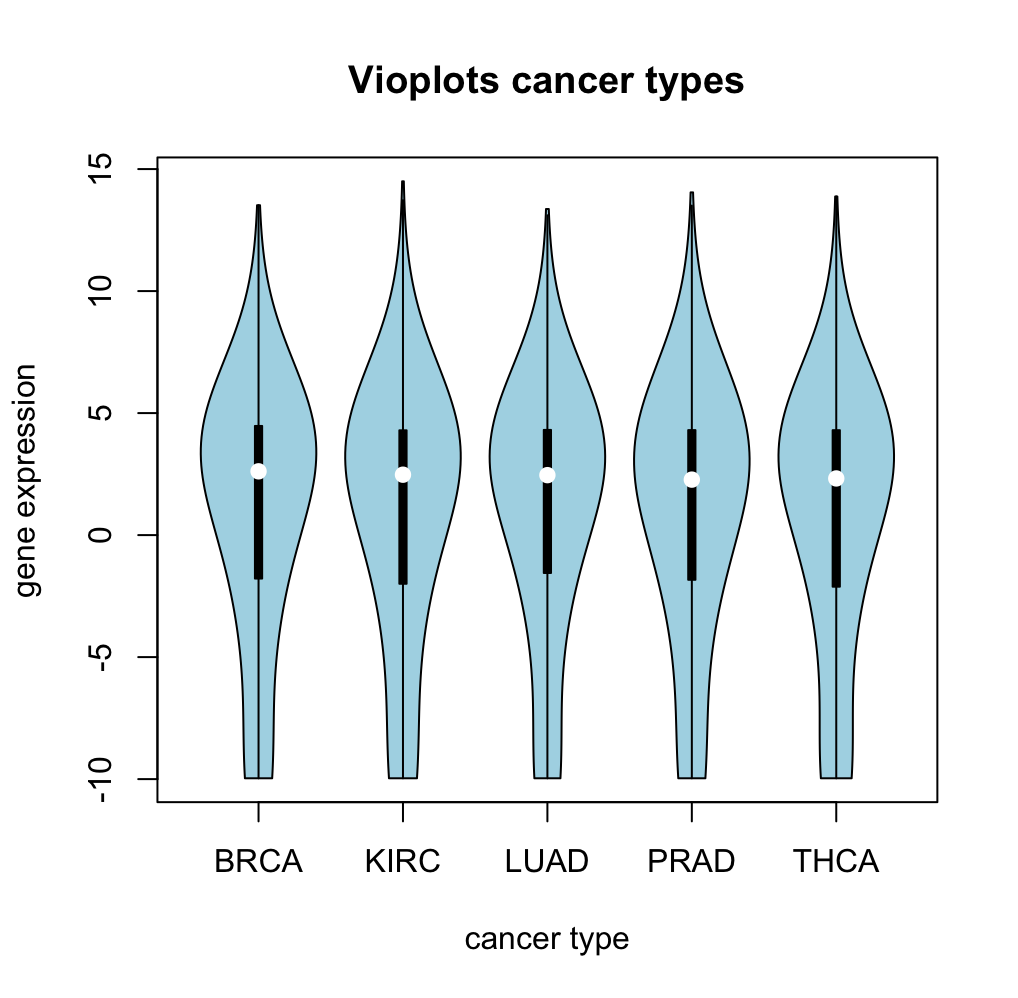
\includegraphics[width=0.3\linewidth]{figures/Vioplots cancer types} 

}

\caption{Mean-variance plot of cleaned TCGA expression data}\label{fig:showviolinplots}
\end{figure}

\hypertarget{packages}{%
\section{Packages}\label{packages}}

\begin{verbatim}
## Warning: Paket 'readxl' wurde unter R Version 4.1.3 erstellt
\end{verbatim}

\begin{table}[!ht]
    \centering
    \caption{Packages used in the analysis.}
    \begin{tabular}{|m{3cm}|m{3cm}|m{5cm}|m{5cm}|}
    \hline
        Package  & Localisation & Usage & Link \\ \hline
        biomart & pre\_02, pre\_03, pre\_05 & renaming the genenames from the hallmarkpathways-dataframe into ensembleIDs & https://bioconductor.org/packages/release/bioc/html/biomaRt.html \\ \hline
        msigdbr & pre\_03 & downloading all of the canonical pathways and the genes which they include in homo sapiens from the msigbdr data base & https://bioconductor.org/packages/release/data/experiment/html/msigdb.html \\ \hline
        dplyr & pre\_04, pre\_05 & tidying and manipulating of dataframes & https://cran.r-project.org/web/packages/dplyr/index.html \\ \hline
        ggplot2 & pre\_04, pre\_05, descr\_03, descr\_04, THCA\_01, THCA\_02, pan\_02, pan\_04 & allows for the creation of plots with more detailed options & https://cran.r-project.org/web/packages/ggplot2/index.html \\ \hline
        pheatmap & descr\_01, pan\_01, neu\_02, neu\_04 & allows for the creation of heatmaps with more detailed options & https://cran.r-project.org/web/packages/pheatmap/pheatmap.pdf \\ \hline
        vioplot & descr\_02 & creation of violinplots & https://cran.r-project.org/web/packages/vioplot/index.html \\ \hline
        VennDiagram & descr\_05 & creation of VENN-diagrams & https://cran.r-project.org/web/packages/VennDiagram/VennDiagram.pdf \\ \hline
        dplyr & THCA\_01, pan\_01 & ~ & ~ \\ \hline
        fgsea & THCA\_01, pan\_01 & to do a GSEA & https://bioconductor.org/packages/release/bioc/html/fgsea.html \\ \hline
        GSVA & THCA\_01, pan\_03 & to do a GSVA & https://bioconductor.org/packages/release/bioc/html/GSVA.html \\ \hline
        ComplexHeatmap & THCA\_01, pan\_03, pan\_04 & allows for the creation of heatmaps with more detailed options & https://bioconductor.org/packages/release/bioc/html/ComplexHeatmap.html \\ \hline
        metaplot & THCA\_02, pan\_02, pan\_04 & data-driven plots & https://cran.r-project.org/web/packages/metaplot/index.html \\ \hline
        gridExtra & THCA\_02, pan\_02, pan\_04 & "implementation of ""grid"" graphics " & https://cran.r-project.org/web/packages/gridExtra/index.html \\ \hline
        umap & THCA\_02, pan\_02, pan\_04 & to do a UMAP & https://cran.r-project.org/web/packages/umap/index.html \\ \hline
        gage & pan\_01 & application of GSEA & https://bioconductor.org/packages/release/bioc/html/gage.html \\ \hline
        psych & pan\_02 & iterative factor analysis & https://cran.r-project.org/web/packages/psych/index.html \\ \hline
        cluster & pan\_04 & cluster analysis & https://cran.r-project.org/web/packages/cluster/cluster.pdf \\ \hline
        MASS & neu\_00 & implementation of neural network & https://cran.r-project.org/web/packages/MASS/index.html \\ \hline
        neuralnet & neu\_03 & training of neural networks & https://cran.r-project.org/web/packages/neuralnet/neuralnet.pdf \\ \hline
        AnnotationDbi & descr\_03 & translating ensemble ids into gennames  & https://bioconductor.org/packages/release/bioc/html/AnnotationDbi.html \\ \hline
        org.Hs.eg.db & descr\_03 & translating ensemble ids into gennames  & https://bioconductor.org/packages/release/data/annotation/html/org.Hs.eg.db.html \\ \hline
    \end{tabular}
\end{table}

\begin{longtable}[]{@{}
  >{\raggedright\arraybackslash}p{(\columnwidth - 6\tabcolsep) * \real{0.07}}
  >{\raggedright\arraybackslash}p{(\columnwidth - 6\tabcolsep) * \real{0.53}}
  >{\raggedright\arraybackslash}p{(\columnwidth - 6\tabcolsep) * \real{0.04}}
  >{\raggedright\arraybackslash}p{(\columnwidth - 6\tabcolsep) * \real{0.36}}@{}}
\caption{Packages used in the analysis.}\tabularnewline
\toprule
\begin{minipage}[b]{\linewidth}\raggedright
Package
\end{minipage} & \begin{minipage}[b]{\linewidth}\raggedright
Usage
\end{minipage} & \begin{minipage}[b]{\linewidth}\raggedright
Authors
\end{minipage} & \begin{minipage}[b]{\linewidth}\raggedright
Link
\end{minipage} \\
\midrule
\endfirsthead
\toprule
\begin{minipage}[b]{\linewidth}\raggedright
Package
\end{minipage} & \begin{minipage}[b]{\linewidth}\raggedright
Usage
\end{minipage} & \begin{minipage}[b]{\linewidth}\raggedright
Authors
\end{minipage} & \begin{minipage}[b]{\linewidth}\raggedright
Link
\end{minipage} \\
\midrule
\endhead
biomart & renaming the genenames from the hallmarkpathways-dataframe
into ensembleIDs & NA &
\url{https://bioconductor.org/packages/release/bioc/html/biomaRt.html} \\
msigdbr & downloading all of the canonical pathways and the genes which
they include in homo sapiens from the msigbdr data base & NA &
\url{https://bioconductor.org/packages/release/data/experiment/html/msigdb.html} \\
dplyr & tidying and manipulating of dataframes & NA &
\url{https://cran.r-project.org/web/packages/dplyr/index.html} \\
ggplot2 & allows for the creation of plots with more detailed options &
NA & \url{https://cran.r-project.org/web/packages/ggplot2/index.html} \\
pheatmap & allows for the creation of heatmaps with more detailed
options & NA &
\url{https://cran.r-project.org/web/packages/pheatmap/pheatmap.pdf} \\
vioplot & creation of violinplots & NA &
\url{https://cran.r-project.org/web/packages/vioplot/index.html} \\
VennDiagram & creation of VENN-diagrams & NA &
\url{https://cran.r-project.org/web/packages/VennDiagram/VennDiagram.pdf} \\
dplyr & NA & NA & NA \\
fgsea & to do a GSEA & NA &
\url{https://bioconductor.org/packages/release/bioc/html/fgsea.html} \\
GSVA & to do a GSVA & NA &
\url{https://bioconductor.org/packages/release/bioc/html/GSVA.html} \\
ComplexHeatmap & allows for the creation of heatmaps with more detailed
options & NA &
\url{https://bioconductor.org/packages/release/bioc/html/ComplexHeatmap.html} \\
metaplot & data-driven plots & NA &
\url{https://cran.r-project.org/web/packages/metaplot/index.html} \\
gridExtra & implementation of ``grid'' graphics & NA &
\url{https://cran.r-project.org/web/packages/gridExtra/index.html} \\
umap & to do a UMAP & NA &
\url{https://cran.r-project.org/web/packages/umap/index.html} \\
gage & application of GSEA & NA &
\url{https://bioconductor.org/packages/release/bioc/html/gage.html} \\
psych & iterative factor analysis & NA &
\url{https://cran.r-project.org/web/packages/psych/index.html} \\
cluster & cluster analysis & NA &
\url{https://cran.r-project.org/web/packages/cluster/cluster.pdf} \\
MASS & implementation of neural network & NA &
\url{https://cran.r-project.org/web/packages/MASS/index.html} \\
neuralnet & training of neural networks & NA &
\url{https://cran.r-project.org/web/packages/neuralnet/neuralnet.pdf} \\
AnnotationDbi & translating ensemble ids into gennames & NA &
\url{https://bioconductor.org/packages/release/bioc/html/AnnotationDbi.html} \\
org.Hs.eg.db & translating ensemble ids into gennames & NA &
\url{https://bioconductor.org/packages/release/data/annotation/html/org.Hs.eg.db.html} \\
\bottomrule
\end{longtable}

\begin{table}

\caption{\label{tab:unnamed-chunk-7}Packages used in the analysis.}
\centering
\begin{tabular}[t]{l|l|l|l}
\hline
Package & Usage & Authors & Link\\
\hline
biomart & renaming the genenames from the hallmarkpathways-dataframe into ensembleIDs & NA & https://bioconductor.org/packages/release/bioc/html/biomaRt.html\\
\hline
msigdbr & downloading all of the canonical pathways and the genes which they include in homo sapiens from the msigbdr data base & NA & https://bioconductor.org/packages/release/data/experiment/html/msigdb.html\\
\hline
dplyr & tidying and manipulating of dataframes & NA & https://cran.r-project.org/web/packages/dplyr/index.html\\
\hline
ggplot2 & allows for the creation of plots with more detailed options & NA & https://cran.r-project.org/web/packages/ggplot2/index.html\\
\hline
pheatmap & allows for the creation of heatmaps with more detailed options & NA & https://cran.r-project.org/web/packages/pheatmap/pheatmap.pdf\\
\hline
vioplot & creation of violinplots & NA & https://cran.r-project.org/web/packages/vioplot/index.html\\
\hline
VennDiagram & creation of VENN-diagrams & NA & https://cran.r-project.org/web/packages/VennDiagram/VennDiagram.pdf\\
\hline
dplyr & NA & NA & NA\\
\hline
fgsea & to do a GSEA & NA & https://bioconductor.org/packages/release/bioc/html/fgsea.html\\
\hline
GSVA & to do a GSVA & NA & https://bioconductor.org/packages/release/bioc/html/GSVA.html\\
\hline
ComplexHeatmap & allows for the creation of heatmaps with more detailed options & NA & https://bioconductor.org/packages/release/bioc/html/ComplexHeatmap.html\\
\hline
metaplot & data-driven plots & NA & https://cran.r-project.org/web/packages/metaplot/index.html\\
\hline
gridExtra & implementation of "grid" graphics & NA & https://cran.r-project.org/web/packages/gridExtra/index.html\\
\hline
umap & to do a UMAP & NA & https://cran.r-project.org/web/packages/umap/index.html\\
\hline
gage & application of GSEA & NA & https://bioconductor.org/packages/release/bioc/html/gage.html\\
\hline
psych & iterative factor analysis & NA & https://cran.r-project.org/web/packages/psych/index.html\\
\hline
cluster & cluster analysis & NA & https://cran.r-project.org/web/packages/cluster/cluster.pdf\\
\hline
MASS & implementation of neural network & NA & https://cran.r-project.org/web/packages/MASS/index.html\\
\hline
neuralnet & training of neural networks & NA & https://cran.r-project.org/web/packages/neuralnet/neuralnet.pdf\\
\hline
AnnotationDbi & translating ensemble ids into gennames & NA & https://bioconductor.org/packages/release/bioc/html/AnnotationDbi.html\\
\hline
org.Hs.eg.db & translating ensemble ids into gennames & NA & https://bioconductor.org/packages/release/data/annotation/html/org.Hs.eg.db.html\\
\hline
\end{tabular}
\end{table}

\hypertarget{code}{%
\section{Code}\label{code}}

world

\begin{Shaded}
\begin{Highlighting}[]
\CommentTok{\#createn einer liste mit allen patienten in dfs sortiert nach krebs}
\NormalTok{cancers }\OtherTok{=} \FunctionTok{list}\NormalTok{();cancers }\OtherTok{=} \FunctionTok{vector}\NormalTok{(}\StringTok{\textquotesingle{}list\textquotesingle{}}\NormalTok{,}\FunctionTok{length}\NormalTok{(}\FunctionTok{table}\NormalTok{(tcga\_anno}\SpecialCharTok{$}\NormalTok{cancer\_type\_abbreviation)))}
\FunctionTok{names}\NormalTok{(cancers) }\OtherTok{=} \FunctionTok{names}\NormalTok{(}\FunctionTok{table}\NormalTok{(tcga\_anno}\SpecialCharTok{$}\NormalTok{cancer\_type\_abbreviation))}
\NormalTok{i}\OtherTok{=}\DecValTok{1}
\ControlFlowTok{for}\NormalTok{ (i }\ControlFlowTok{in} \DecValTok{1}\SpecialCharTok{:}\FunctionTok{length}\NormalTok{(cancers))\{}
\NormalTok{  cancers[[i]] }\OtherTok{=}\NormalTok{ tcga\_exp\_cleaned[,tcga\_anno}\SpecialCharTok{$}\NormalTok{cancer\_type\_abbreviation }\SpecialCharTok{==} \FunctionTok{names}\NormalTok{(cancers)[i]]}
\NormalTok{\}}
\CommentTok{\#function die einen krebstypen df und genesets als input nimmt und ein df mit pvalues ausgibt}
\NormalTok{enrichment }\OtherTok{=} \ControlFlowTok{function}\NormalTok{(expressiondata, }\AttributeTok{genesets =}\NormalTok{ genesets\_ids)\{}
\NormalTok{  ESmatrix }\OtherTok{=} \FunctionTok{sapply}\NormalTok{(genesets, }\AttributeTok{FUN =} \ControlFlowTok{function}\NormalTok{(x)\{}
\NormalTok{    ins }\OtherTok{=} \FunctionTok{na.omit}\NormalTok{(}\FunctionTok{match}\NormalTok{(x,}\FunctionTok{rownames}\NormalTok{(expressiondata)))}\CommentTok{\#indices der gene im aktuellen set}
\NormalTok{    outs }\OtherTok{=} \SpecialCharTok{{-}}\NormalTok{ins}\CommentTok{\#indices der gene nicht im aktuellen set}
    \CommentTok{\#gibt einen vektor der für jeden patienten den pval für das aktuelle gene enthält}
\NormalTok{    res }\OtherTok{=} \ConstantTok{NULL}
    \ControlFlowTok{for}\NormalTok{ (i }\ControlFlowTok{in} \DecValTok{1}\SpecialCharTok{:}\FunctionTok{ncol}\NormalTok{(expressiondata))\{}\CommentTok{\#testet für jeden patienten}
\NormalTok{      res[i] }\OtherTok{=} \FunctionTok{wilcox.test}\NormalTok{(expressiondata[ins,i],expressiondata[outs,i],}\StringTok{\textquotesingle{}two.sided\textquotesingle{}}\NormalTok{)}\SpecialCharTok{$}\NormalTok{p.value}
\NormalTok{    \}}
    \FunctionTok{return}\NormalTok{(res)}
\NormalTok{  \})}
  \FunctionTok{row.names}\NormalTok{(ESmatrix) }\OtherTok{=} \FunctionTok{colnames}\NormalTok{(expressiondata); }\FunctionTok{return}\NormalTok{(ESmatrix)}
\NormalTok{\}}
\NormalTok{pvalueslist }\OtherTok{=} \FunctionTok{lapply}\NormalTok{(cancers, enrichment)}\CommentTok{\#für die tests für jeden krebstypen durch}
\end{Highlighting}
\end{Shaded}

\begin{Shaded}
\begin{Highlighting}[]
\NormalTok{get\_top10pathways\_from\_pvalues }\OtherTok{=} \ControlFlowTok{function}\NormalTok{(df\_p\_values, length\_genesets) \{}
  
  \FunctionTok{require}\NormalTok{(ggplot2)}
  
\NormalTok{  results }\OtherTok{\textless{}{-}} \FunctionTok{list}\NormalTok{()}
    
\NormalTok{  df\_p\_values\_log10 }\OtherTok{\textless{}{-}} \SpecialCharTok{{-}}\FunctionTok{log10}\NormalTok{(}\FunctionTok{as.data.frame}\NormalTok{(df\_p\_values))}
    
\NormalTok{  mean\_pathway }\OtherTok{\textless{}{-}} \FunctionTok{as.data.frame}\NormalTok{(}\FunctionTok{apply}\NormalTok{(df\_p\_values\_log10, }\DecValTok{1}\NormalTok{, mean))}
  \FunctionTok{rownames}\NormalTok{(mean\_pathway) }\OtherTok{\textless{}{-}} \FunctionTok{rownames}\NormalTok{(df\_p\_values\_log10)}
  
\NormalTok{  ordered\_score }\OtherTok{\textless{}{-}}\NormalTok{ mean\_pathway[}\FunctionTok{order}\NormalTok{(}\SpecialCharTok{{-}}\NormalTok{mean\_pathway[ ,}\DecValTok{1}\NormalTok{]), }\DecValTok{1}\NormalTok{]}
\NormalTok{  top\_10 }\OtherTok{\textless{}{-}} \FunctionTok{data.frame}\NormalTok{(ordered\_score[}\DecValTok{1}\SpecialCharTok{:}\DecValTok{10}\NormalTok{])}
  \FunctionTok{colnames}\NormalTok{(top\_10) }\OtherTok{\textless{}{-}} \StringTok{"mean\_pathway"}
  
\NormalTok{  ordered\_names }\OtherTok{\textless{}{-}} \FunctionTok{order}\NormalTok{(}\SpecialCharTok{{-}}\NormalTok{mean\_pathway[ ,}\DecValTok{1}\NormalTok{])}
\NormalTok{  top\_10\_names }\OtherTok{\textless{}{-}}\NormalTok{ ordered\_names[}\DecValTok{1}\SpecialCharTok{:}\DecValTok{10}\NormalTok{]}
\NormalTok{  top\_10}\SpecialCharTok{$}\NormalTok{pathway\_names }\OtherTok{\textless{}{-}} \FunctionTok{row.names}\NormalTok{(mean\_pathway)[top\_10\_names]}
  
\NormalTok{  results[[}\DecValTok{1}\NormalTok{]] }\OtherTok{\textless{}{-}}\NormalTok{ top\_10}
  
\NormalTok{  results[[}\DecValTok{2}\NormalTok{]] }\OtherTok{\textless{}{-}} \FunctionTok{ggplot}\NormalTok{(}\AttributeTok{data =}\NormalTok{ top\_10, }\FunctionTok{aes}\NormalTok{(}\AttributeTok{x =}\NormalTok{ mean\_pathway, }\AttributeTok{y =} \FunctionTok{reorder}\NormalTok{(pathway\_names, mean\_pathway)))}\SpecialCharTok{+}
    \FunctionTok{geom\_bar}\NormalTok{(}\AttributeTok{stat =} \StringTok{"identity"}\NormalTok{)}\SpecialCharTok{+}
    \FunctionTok{coord\_cartesian}\NormalTok{(}\AttributeTok{xlim =}\FunctionTok{c}\NormalTok{(}\DecValTok{3}\NormalTok{, }\FloatTok{3.75}\NormalTok{))}\SpecialCharTok{+}
    \FunctionTok{labs}\NormalTok{(}\AttributeTok{title =} \FunctionTok{names}\NormalTok{(df\_p\_values),}
         \AttributeTok{x =} \StringTok{"mean p{-}value pathway"}\NormalTok{,}
         \AttributeTok{y =} \StringTok{"pathway name"}\NormalTok{)}
  
\NormalTok{  pathway\_size }\OtherTok{\textless{}{-}} \FunctionTok{order}\NormalTok{(}\SpecialCharTok{{-}}\NormalTok{mean\_pathway[ ,}\DecValTok{1}\NormalTok{])}
\NormalTok{  top\_10\_size }\OtherTok{\textless{}{-}}\NormalTok{ pathway\_size[}\DecValTok{1}\SpecialCharTok{:}\DecValTok{10}\NormalTok{]}
\NormalTok{  top\_10}\SpecialCharTok{$}\NormalTok{pathway\_size }\OtherTok{\textless{}{-}}\NormalTok{ length\_genesets[top\_10\_size]}
  
\NormalTok{  results[[}\DecValTok{3}\NormalTok{]] }\OtherTok{\textless{}{-}} \FunctionTok{ggplot}\NormalTok{(}\AttributeTok{data =}\NormalTok{ top\_10, }\FunctionTok{aes}\NormalTok{(}\AttributeTok{x =}\NormalTok{ mean\_pathway, }\AttributeTok{y =} \FunctionTok{reorder}\NormalTok{(pathway\_names,}
\NormalTok{                                                                          mean\_pathway)))}\SpecialCharTok{+}
    \FunctionTok{geom\_point}\NormalTok{(}\FunctionTok{aes}\NormalTok{(}\AttributeTok{size =}\NormalTok{ pathway\_size))}\SpecialCharTok{+}
    \FunctionTok{labs}\NormalTok{(}\AttributeTok{title =} \FunctionTok{names}\NormalTok{(df\_p\_values),}
         \AttributeTok{x =} \StringTok{"mean p{-}value pathway"}\NormalTok{,}
         \AttributeTok{y =} \StringTok{"pathway name"}\NormalTok{)}
  
  \FunctionTok{return}\NormalTok{(results)}
\NormalTok{\}}
\end{Highlighting}
\end{Shaded}


\end{document}
